\chapter{Secret messages}\label{chapter:RSA}
\begin{epigraphs}
\qitem[author={Sylvia Plath}, source={The Unabridged Journals of Sylvia Plath}]{And when at last you find someone to whom you feel you can pour out your soul, you stop in shock at the words you utter— they are so rusty, so ugly, so meaningless and feeble from being kept in the small cramped dark inside you so long.}\SubIndex{Plath, Sylvia}\SubIndex{The Unabridged Journals of Sylvia Plath}
\qitem[author={André Malraux}]{Man is not what he thinks he is, he is what he hides.}\SubIndex{Malraux, André} 
\end{epigraphs}
\begin{center}
\begin{minipage}{6cm}
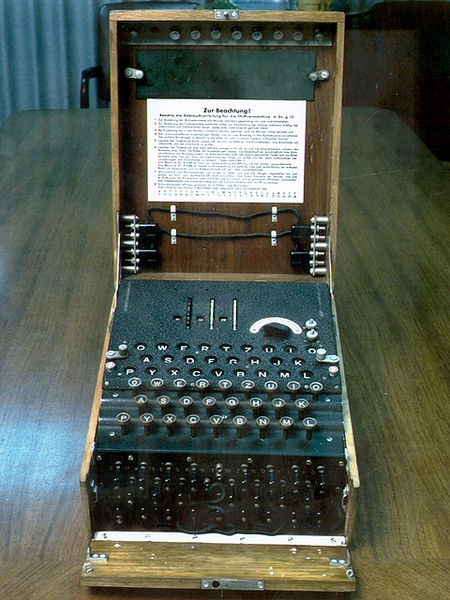
\includegraphics[width=6cm]{Enigma.jpg}
\\
\emph{Enigma},\SubIndex{enigma} Nazi secret code machine
\end{minipage}
\end{center}
\section{RSA: the Cocks, Rivest, Shamir and Adleman algorithm}\SubIndex{RSA algorithm}
\begin{example}
Alice\SubIndex{Alice} wants to send a message to Bob,\SubIndex{Bob} but she doesn't want Eve\SubIndex{Eve} to read it.
She first writes the message down in a computer, as a collection of \(0\)'s and \(1\)'s.
She can think of these \(0\)'s and \(1\)'s as binary digits of some large integer \(x\), or as binary digits of some \emph{remainder}\SubIndex{remainder} \(x\) modulo some large integer \(m\).
Alice takes her message \(x\) and turns it into a secret coded message by sending Bob not the original \(x\), but instead sending him \(x^d\) modulo \(m\), for some integer \(d\).
This will scramble up the digits of \(x\) unrecognizably, if \(d\) is chosen ``at random''.
For random enough \(d\), and suitably chosen positive integer \(m\), Bob can unscramble the digits of \(x^d\) to find \(x\).
\end{example}
\begin{example}
For example, take \(m\defeq 55\) and let \(d\defeq 17\) and \(y\defeq x^{17} \operatorname{mod} 55\):
\[
\begin{array}{@{}rrp{0pt}rrp{0pt}rrp{0pt}rr@{}}
\toprule
x & y && x & y && x & y && x & y \\
\cmidrule(r){1-1}
\cmidrule(lr){2-2}
\cmidrule(lr){4-4}
\cmidrule(lr){5-5}
\cmidrule(lr){7-7}
\cmidrule(lr){8-8}
\cmidrule(lr){10-10}
\cmidrule(l){11-11}
 0 & 0 && 14 & 9 && 28 & 8 && 42 & 37\\ 
 1 & 1 && 15 & 5 && 29 & 39 && 43 & 43\\ 
 2 & 7 && 16 & 36 && 30 & 35 && 44 & 44\\ 
 3 & 53 && 17 & 52 && 31 & 26 && 45 & 45\\ 
 4 & 49 && 18 & 28 && 32 & 32 && 46 & 51\\ 
 5 & 25 && 19 & 24 && 33 & 33 && 47 & 42\\ 
 6 & 41 && 20 & 15 && 34 & 34 && 48 & 38\\ 
 7 & 17 && 21 & 21 && 35 & 40 && 49 & 14\\ 
 8 & 13 && 22 & 22 && 36 & 31 && 50 & 30\\ 
 9 &   4 && 23 & 23 && 37 & 27 && 51 & 6\\ 
 10 & 10 && 24 & 29 && 38 & 3 && 52 & 2\\ 
 11 & 11 && 25 & 20 && 39 & 19 && 53 & 48\\ 
 12 & 12 && 26 & 16 && 40 & 50 && 54 & 54\\ 
 13 & 18 && 27 & 47 && 41 & 46 && 55 & 0\\ 
% s=""
%for i in range(0,14):
%    s=s+"{} & {} & {} & {} & {} & {} & {} & {}".format(i,mod(i,55)^(17),i+14,mod(i+14,55)^(17),i+2*14,mod(i+2*14,55)^(17),i+3*14,mod(i+3*14,55)^(17))+r"\\" + " \n "
%print(s)
%%0 & 0 & 20 & 15 & 40 & 50\\ 
%% 1 & 1 & 21 & 21 & 41 & 46\\ 
%% 2 & 7 & 22 & 22 & 42 & 37\\ 
%% 3 & 53 & 23 & 23 & 43 & 43\\ 
%% 4 & 49 & 24 & 29 & 44 & 44\\ 
%% 5 & 25 & 25 & 20 & 45 & 45\\ 
%% 6 & 41 & 26 & 16 & 46 & 51\\ 
%% 7 & 17 & 27 & 47 & 47 & 42\\ 
%% 8 & 13 & 28 & 8 & 48 & 38\\ 
%% 9 & 4 & 29 & 39 & 49 & 14\\ 
%% 10 & 10 & 30 & 35 & 50 & 30\\ 
%% 11 & 11 & 31 & 26 & 51 & 6\\ 
%% 12 & 12 & 32 & 32 & 52 & 2\\ 
%% 13 & 18 & 33 & 33 & 53 & 48\\ 
%% 14 & 9 & 34 & 34 & 54 & 54\\ 
%% 15 & 5 & 35 & 40 & 55 & 0\\ 
%% 16 & 36 & 36 & 31 & 56 & 1\\ 
%% 17 & 52 & 37 & 27 & 57 & 7\\ 
%% 18 & 28 & 38 & 3 & 58 & 53\\ 
%% 19 & 24 & 39 & 19 & 59 & 49\\
%0  &  0  &  28  &  8 \\
%1  &  1  &  29  &  39 \\
%2  &  7  &  30  &  35 \\
%3  &  53  &  31  &  26 \\
%4  &  49  &  32  &  32 \\
%5  &  25  &  33  &  33 \\
%6  &  41  &  34  &  34 \\
%7  &  17  &  35  &  40 \\
%8  &  13  &  36  &  31 \\
%9  &  4  &  37  &  27 \\
%10  &  10  &  38  &  3 \\
%11  &  11  &  39  &  19 \\
%12  &  12  &  40  &  50 \\
%13  &  18  &  41  &  46 \\
%14  &  9  &  42  &  37 \\
%15  &  5  &  43  &  43 \\
%16  &  36  &  44  &  44 \\
%17  &  52  &  45  &  45 \\
%18  &  28  &  46  &  51 \\
%19  &  24  &  47  &  42 \\
%20  &  15  &  48  &  38 \\
%21  &  21  &  49  &  14 \\
%22  &  22  &  50  &  30 \\
%23  &  23  &  51  &  6 \\
%24  &  29  &  52  &  2 \\
%25  &  20  &  53  &  48 \\
%26  &  16  &  54  &  54 \\
%27  &  47  &  55  &  0 \\
\bottomrule
\end{array}
\]
%\[
%\begin{array}{@{}rr@{\hspace{1cm}}rr@{\hspace{1cm}}rr@{\hspace{1cm}}rr@{}}
%\toprule
%x & y & x & y & x & y & x & y \\
%\cmidrule(r){1-1}
%\cmidrule(lr{1cm}){2-2}
%\cmidrule(lr){3-3}
%\cmidrule(lr{1cm}){4-4}
%\cmidrule(lr){5-5}
%\cmidrule(lr{1cm}){6-6}
%\cmidrule(lr){7-7}
%\cmidrule(l){8-8}
%0 & 0 & 14 & 9 & 28 & 8 & 42 & 37\\ 
% 1 & 1 & 15 & 5 & 29 & 39 & 43 & 43\\ 
% 2 & 7 & 16 & 36 & 30 & 35 & 44 & 44\\ 
% 3 & 53 & 17 & 52 & 31 & 26 & 45 & 45\\ 
% 4 & 49 & 18 & 28 & 32 & 32 & 46 & 51\\ 
% 5 & 25 & 19 & 24 & 33 & 33 & 47 & 42\\ 
% 6 & 41 & 20 & 15 & 34 & 34 & 48 & 38\\ 
% 7 & 17 & 21 & 21 & 35 & 40 & 49 & 14\\ 
% 8 & 13 & 22 & 22 & 36 & 31 & 50 & 30\\ 
% 9 & 4 & 23 & 23 & 37 & 27 & 51 & 6\\ 
% 10 & 10 & 24 & 29 & 38 & 3 & 52 & 2\\ 
% 11 & 11 & 25 & 20 & 39 & 19 & 53 & 48\\ 
% 12 & 12 & 26 & 16 & 40 & 50 & 54 & 54\\ 
% 13 & 18 & 27 & 47 & 41 & 46 & 55 & 0\\ 
%% s=""
%%for i in range(0,14):
%%    s=s+"{} & {} & {} & {} & {} & {} & {} & {}".format(i,mod(i,55)^(17),i+14,mod(i+14,55)^(17),i+2*14,mod(i+2*14,55)^(17),i+3*14,mod(i+3*14,55)^(17))+r"\\" + " \n "
%%print(s)
%%%0 & 0 & 20 & 15 & 40 & 50\\ 
%%% 1 & 1 & 21 & 21 & 41 & 46\\ 
%%% 2 & 7 & 22 & 22 & 42 & 37\\ 
%%% 3 & 53 & 23 & 23 & 43 & 43\\ 
%%% 4 & 49 & 24 & 29 & 44 & 44\\ 
%%% 5 & 25 & 25 & 20 & 45 & 45\\ 
%%% 6 & 41 & 26 & 16 & 46 & 51\\ 
%%% 7 & 17 & 27 & 47 & 47 & 42\\ 
%%% 8 & 13 & 28 & 8 & 48 & 38\\ 
%%% 9 & 4 & 29 & 39 & 49 & 14\\ 
%%% 10 & 10 & 30 & 35 & 50 & 30\\ 
%%% 11 & 11 & 31 & 26 & 51 & 6\\ 
%%% 12 & 12 & 32 & 32 & 52 & 2\\ 
%%% 13 & 18 & 33 & 33 & 53 & 48\\ 
%%% 14 & 9 & 34 & 34 & 54 & 54\\ 
%%% 15 & 5 & 35 & 40 & 55 & 0\\ 
%%% 16 & 36 & 36 & 31 & 56 & 1\\ 
%%% 17 & 52 & 37 & 27 & 57 & 7\\ 
%%% 18 & 28 & 38 & 3 & 58 & 53\\ 
%%% 19 & 24 & 39 & 19 & 59 & 49\\
%%0  &  0  &  28  &  8 \\
%%1  &  1  &  29  &  39 \\
%%2  &  7  &  30  &  35 \\
%%3  &  53  &  31  &  26 \\
%%4  &  49  &  32  &  32 \\
%%5  &  25  &  33  &  33 \\
%%6  &  41  &  34  &  34 \\
%%7  &  17  &  35  &  40 \\
%%8  &  13  &  36  &  31 \\
%%9  &  4  &  37  &  27 \\
%%10  &  10  &  38  &  3 \\
%%11  &  11  &  39  &  19 \\
%%12  &  12  &  40  &  50 \\
%%13  &  18  &  41  &  46 \\
%%14  &  9  &  42  &  37 \\
%%15  &  5  &  43  &  43 \\
%%16  &  36  &  44  &  44 \\
%%17  &  52  &  45  &  45 \\
%%18  &  28  &  46  &  51 \\
%%19  &  24  &  47  &  42 \\
%%20  &  15  &  48  &  38 \\
%%21  &  21  &  49  &  14 \\
%%22  &  22  &  50  &  30 \\
%%23  &  23  &  51  &  6 \\
%%24  &  29  &  52  &  2 \\
%%25  &  20  &  53  &  48 \\
%%26  &  16  &  54  &  54 \\
%%27  &  47  &  55  &  0 \\
%\bottomrule
%\end{array}
%\]
If Alice sends Bob the secret message \(y=x^{17}\), then Bob decodes it by \(x=y^{33}\), as we will see.
\end{example}
\begin{theorem}\label{theorem:RSA}
Pick two different prime numbers \(p\) and \(q\) and let \(m\defeq pq\).
Recall Euler's totient\SubIndex{Euler's totient function} function \(\phi(m)\).
Suppose that \(d\) and \(e\) are positive integers so that \(de=1\) modulo \(\phi(m)\).
If Alice maps each remainder \(x\) to \(y=x^d\) modulo \(m\), then Bob can invert this map by taking each remainder \(y\) to \(x=y^e\) modulo \(m\).
\end{theorem}
\begin{proof}
We have to prove that \(\pr{x^d}^e=x\) modulo \(m\) for all \(x\), i.e. that \(x^{de}=x\) modulo \(m\) for all \(x\).
For \(x\) coprime to \(m\), this follows from Euler's theorem, but for other values of \(x\) the result is not obvious.

By theorem~\vref{theorem:totient}, \(\phi(m)=(p-1)(q-1)\).
Since \(de=1\) modulo \(\phi(m)\), clearly 
\[
de-1=k(p-1)(q-1)
\]
for some integer \(k\).
If \(k=0\), then \(de=1\) and the result is clear: \(x^1=x\).
Since \(d\) and \(e\) are positive integers, \(de-1\) is not negative, so \(k \ge 0\).
So we can assume that \(k>0\).
The result follows from theorem~\vref{theorem:generalized.Euler}.
\end{proof}
\begin{problem}{rsa:encode}
Take each letter in the alphabet, ordered 
\[
abc\dots{}zABC\dots{}Z,
\]
and one ``blank space'' letter \underline{\phantom{X}}, so \(26+26+1=53\) letters in all.
Use the rule that each letter is then represented by a number from \(100\) to \(152\), starting with \(a \mapsto 100\), \(b \mapsto 101\), and so on to \(\textrm{\underline{\phantom{X}}} \mapsto 152\).
Then string the digits of these numbers together into a single number.
For example, \(ab\underline{\phantom{X}}c\) is \num{100101152102}.
\begin{enumerate}
\item
Write out the message \emph{Hail\underline{\phantom{X}}Caesar} as a number.
\item
Translate the number \num{127114114111104} into letters by this encoding.
\item
Apply the method above, taking
\begin{align*}
p
&= 
\num{993319},
\\
q
&=
\num{999331},
\\
d
&=13
\end{align*}
and use a computer to compute the secret code on the number \(x=127 \, 114 \, 114 \, 111 \, 104\).
You should get:
\[
y=\num{202002770451}
\]
\item
Use a computer to check that the associated number \(e\) for the given numbers \(p,q,d\) in this case is
\[
e=\num{839936711257}.
\]
How can you use a computer to find this number \(e\), if you only know the numbers \(p, q, d\) in this case?
\item
Use the process described in theorem~\vref{theorem:RSA} to decode the message
\[
y=\num{660968731660}.
\]
Warning: you might want to factor \(e\) first and then compute the power \(y^e\) modulo \(m\) by computing one factor of \(e\) at a time.
\end{enumerate}
\end{problem}

\section{Sage}
Sage shines because we can't do any of the computations of this chapter by hand.
\subsection{Alice}
To encode a single letter as a number, sage has a function \verb!ord()!:
\begin{sageblock}
ord('A')
\end{sageblock}
yields \(\sage{ord('A')}\), giving each letter (and punctuation sign and space, etc.) a different positive integer less than 100.
(If Alice wants to use lower case letters, we need to go beyond 100, so let's not do that.)
To apply this to an entire string of text,
\begin{sageblock}
m = "HELLO WORLD"
m = list(map(ord, m))
m
\end{sageblock}
yields
\(\sage{m}\).
Alice turns this list of numbers into a single number, by first reversing order:
\begin{sageblock}
m.reverse()
m
\end{sageblock}
yields
\(\sage{m}\).
Then the expression
\begin{sageblock}
ZZ(m,100)
\end{sageblock}
adds up successively these numbers, multiplying by \(100\) at each step, so that
\begin{sageblock}
x=ZZ(m,100)
x
\end{sageblock}
yields \(x\).
This is the integer Alice wants to encode.
Alice sets up the values of her primes and exponent:
\begin{sageblock}
p=993319
q=999331
d=13
m=p*q
f=euler_phi(m)
e=inverse_mod(d,f)
\end{sageblock}
The secret code Alice sends is \(y=x^d\pmod{m}\).
Sage can compute powers in modular arithmetic quickly (using the same tricks we learned previously):
\begin{sageblock}
y=power_mod(x, d, m)
y
\end{sageblock}
yielding \(\sage{y}\).
This is Alice's encoded message.
She can send it to Bob openly: over the phone, by email, or on a billboard.
\subsection{Bob}
Bob decodes by
\begin{sageblock}
x=power_mod(y, e, m)
x
\end{sageblock}
yielding \(\sage{x}\).
(Alice has secretly whispered \(e\) and \(m\) to Bob.)
Bob turns this number \(x\) back into text by using the function \verb!chr()!, which is the inverse of \verb!ord()!:
\begin{sageblock}
def recover_message(x):
    if x==0:
        return ""
    else:
        return recover_message(x//100)+chr(x%100)
\end{sageblock}
Bob applies this:
\begin{sageblock}
print(recover_message(x))
\end{sageblock}
to yield \verb!HELLO WORLD!.
